\section{Durchführung}
\label{sec:Durchführung}
Für den Versuch wird die in \autoref{fig:aufbau} zu sehende Apparatur genutzt.
\begin{figure}[H]
    \centering
    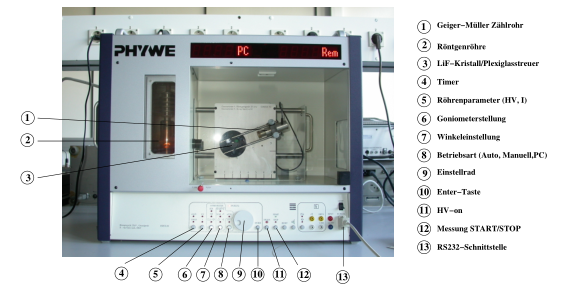
\includegraphics[width=\textwidth]{images/aufbau.PNG}
    \caption{Apparatur zur Erzeugung und Messung von Röntgenstrahlung. \cite{603}}
    \label{fig:aufbau}
\end{figure}
\noindent Die zu sehende Apparatur besteht im Wesentlichen aus einer Röntgenröhre,
einem LiF-Kristall bzw. einem Plexiglasstreuer und einem Geiger-Müller-Zählrohr. Für alle folgenden Messungen werden eine Beschleunigungsspannung von $\SI{35}{\kilo\volt}$ und ein Emissionsstrom von $\SI{1}{\milli\ampere}$ eingestellt.

\subsection{Aufnahme des Emissionsspektrums der Röntgenröhre}
Für die Bestimmung des Emissionsspektrums der Kupfer-Röntgenröhre, wird an der Apparatur das Programm measure ausgewählt. Für die Messung werden eine $\SI{2}{\milli\meter}$-Blende und der LiF-Kristall in die Apparatur eingebaut.
Dann wird der Winkel des LiF-Kristalls in Schritten von $\symup{\Delta}\alpha = \SI{0.1}{\degree}$, bei einer Integrationszeit von $t = \SI{10}{\second}$, erhöht .

\subsection{Experimentelle Bestimmung der Transmission und der Compton-Wellenlänge}
Nun wird die Transmission $T(\lambda)$ eines Aluminium-Absorbers bestimmt.
    Dazu wird der Absorber vor der Blende befestigt und  es wird in einem Intervall von $\alpha = [\SI{7}{\degree}, \SI{10}{\degree}]$ in Schritten von $\symup{\Delta}\alpha = \SI{0.1}{\degree}$ mit Integrationszeit $t = \SI{200}{\second}$ die Zählrate gemessen.
    Dabei wird sowohl die Zählrate ohne Absorber $N_0(\alpha)$, als auch die Zählrate mit Absorber $N_\text{Al}(\alpha)$ gemessen.

    \noindent Aufgrund der Totzeit des Geiger-Müller-Zählrohrs $\tau = \SI{90}{\micro\second}$
    muss eine Totzeitkorrektur nach
    \begin{equation}
        I = \frac{N}{1 - \tau N} 
        \label{eqn:totzeitkorrektur}
    \end{equation}
    \noindent vorgenommen werden.
    \\
    Die weiteren Messungen werden manuell ohne das Rechnerprogramm durchgeführt.
    Für den manuellen Betrieb wird das Röntgengerät auf Manuell umgeschaltet und das RS232-Kabel entfernt.\\
    \\
    Im nächsten Schritt wird die 2 mm Blende durch eine 5 mm Blende und der LiF-Kristall
    durch den Plexiglas-Streuer ersetzt. Dann wird der Kristall auf $\SI{45}{\degree}$ und das Geiger-Müller
    Zählrohr auf $\SI{90}{\degree}$ (siehe \autoref{fig:aufbauab}) gestellt und die Intensität $I_0$ der Cu-Röhre gemessen.

    \begin{figure}[H]
        \centering
        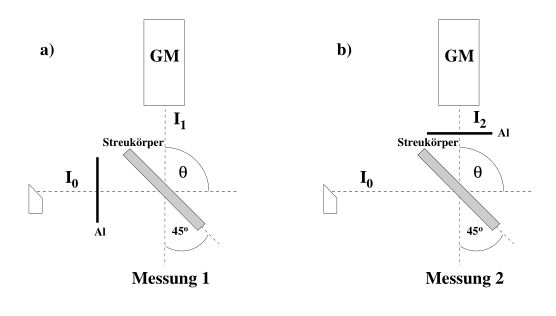
\includegraphics[width=0.75\textwidth]{images/aufbauab.jpg}
        \caption{Aufbau für die Bestimmung der Compton-Wellenlänge. \cite{603}}
        \label{fig:aufbauab}
    \end{figure}    

    \noindent Nun wird zuerst die Transmission $T_1 = \sfrac{I_1}{I_0}$ der ungestreuten Wellenlänge $\lambda_1$ gemessen, indem der Absorber zwischen Röntgenröhre und Plexiglasstreuer eingebaut wird (\autoref{fig:aufbauab}a).
    
    \noindent Für die gestreute Röntgenstrahlung mit Wellenlänge $\lambda_2$ wird anschließend die Transmission $T_2 = \sfrac{I_2}{I_0}$ bestimmt, indem der Aluminium-Absorber nach \autoref{fig:aufbauab}b
    zwischen Plexiglasstreuer und Geiger-Müller-Zählrohr gebracht wird. 
    
    \noindent Bei der Bestimmung der Transmissionen wird jeweils mit einer Integrationszeit von $t = \SI{300}{\second}$ gemessen.